\chapter{Arquitectura del sistema}

El sistema se ha dividido en dos módulos: la plataforma aérea y la estación de tierra. La plataforma aérea está compuesta 
por el propio UAV y una Jetson Nano, que actúa como pasarela de comunicación entre el UAV y la estación de tierra.

Esta pasarela adquiere la información visual e inercial procedente de la cámara a bordo, una Intel RealSense D435i, y la separa 
en tres canales. El canal de profundidad se almacena en una tarjeta SD para su posterior comparación y validación con el algoritmo 
de navegación. El canal visual se reenvía mediante un flujo RTSP a través de Wi-Fi hasta la estación de tierra, con el objetivo de 
minimizar la latencia y maximizar el rendimiento. Finalmente, el canal inercial, correspondiente a la IMU, se envía mediante un 
socket UDP hasta la estación de tierra. De esta forma, se gestionan adecuadamente las distintas frecuencias de muestreo empleadas 
por cada uno de los sensores.

En la Figura \ref{fig:plataforma_aerea} se muestra la arquitectura general de la plataforma aérea.

\begin{figure}[H]
    \ffigbox[\FBwidth] {
        \caption[Arquitectura de la plataforma aérea]{Arquitectura de la plataforma aérea.}
        \label{fig:plataforma_aerea}
    }
    {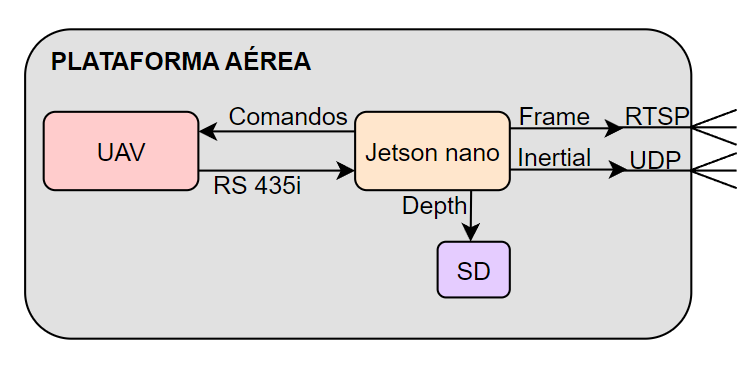
\includegraphics[scale=0.7]{images/plataforma_aerea.png}}
\end{figure}

En la estación de tierra se ejecuta el algoritmo de navegación, aprovechando la capacidad de cómputo de un ordenador central más 
potente que el sistema embarcado. Esta estación recibe la información visual e inercial procedente de la plataforma aérea y la 
adapta para ser utilizada como entrada del algoritmo de navegación. Además, el sistema recibe como entrada un conjunto de 
\textit{waypoints} definidos por el usuario.

En primer lugar, los canales visual e inercial se procesan mediante un sistema de odometría visual-inercial, encargado de estimar 
la pose del UAV respecto al punto de inicio del algoritmo. De forma paralela, el canal visual se introduce en un estimador de 
profundidad que, junto con un algoritmo de evitación de obstáculos, proporciona una dirección de movimiento segura.

Toda esta información, junto con la trayectoria generada por el planificador global, se introduce en un planificador local. Este 
genera las referencias necesarias para un controlador PID, encargado de obtener el control en velocidad del dron. Finalmente, el 
comando de velocidad, compuesto por sus componentes lineal y angular, se envía mediante UDP de vuelta al dron para su ejecución.

En la Figura \ref{fig:estacion_tierra} se muestra la arquitectura general de la estación de tierra.


\begin{figure}[H]
    \ffigbox[\FBwidth] {
        \caption[Arquitectura de la estación de tierra]{Arquitectura de la estación de tierra.}
        \label{fig:estacion_tierra}
    }
    {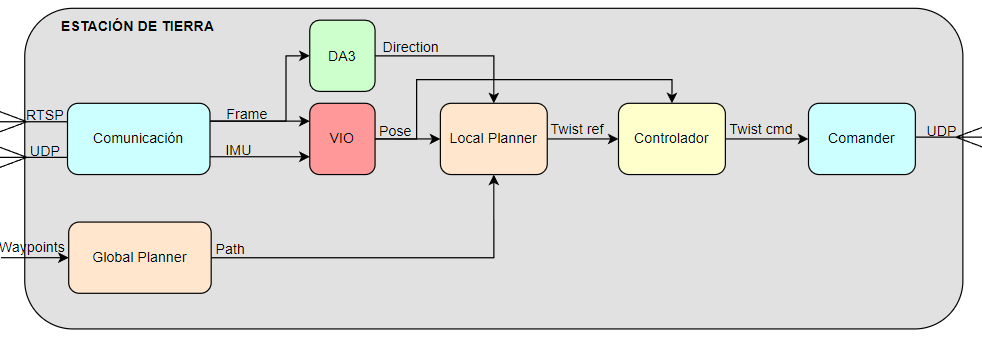
\includegraphics[scale=0.55]{images/estacion_tierra.png}}
\end{figure}

\section{Descripción de componentes del sistema}

La plataforma aérea cuenta con un controlador de vuelo Orange Cube, mostrado en la Figura~\ref{fig:orange_cube}. Este dispositivo 
se encarga del control de bajo nivel del UAV y permite comandar la plataforma mediante consignas de velocidad y actitud. Sus 
características principales son:

\begin{figure}[H]
    \ffigbox[\FBwidth] {
        \caption[Controlador Orange Cube]{Controlador Orange Cube.}
        \label{fig:orange_cube}
    }
    {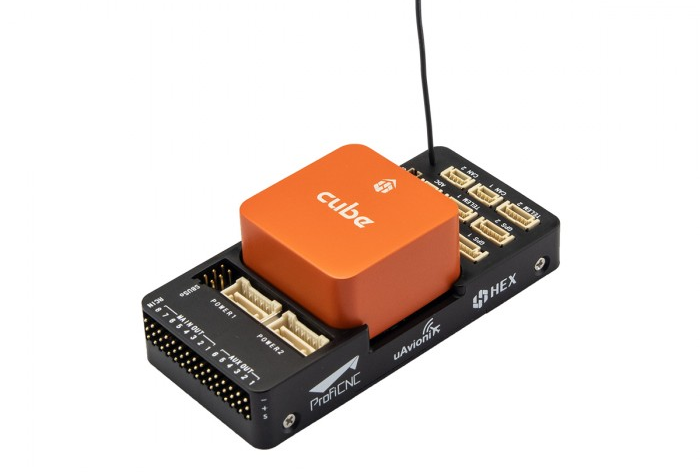
\includegraphics[scale=0.45]{images/orange_cube.png}}
\end{figure}

\begin{itemize}[nosep]
    \item Procesador STM32H753 Cortex\textsuperscript{\textregistered}-M7 con 1 MB de RAM y 2 MB de Flash.
    \item 1 IMU InvenSense ICM20602 y 1 IMU ICM20948.
    \item 2 barómetros MS5611.
    \item 1 magnetómetro AK09916.
    \item 1 acelerómetro y giroscopio ICM20649.
    \item Varios sensores de temperatura y conexión para GPS.
    \item 2 conectores para recepción de telemetría mediante protocolo UART.
\end{itemize}

En este proyecto, los sensores internos del controlador de vuelo no se emplean como fuente principal de percepción para el 
algoritmo de navegación desarrollado. Su uso queda asociado principalmente al control y estabilización de bajo nivel del UAV. El 
objetivo del sistema es lograr una navegación autónoma y una evitación de obstáculos estable a partir de la información visual e 
inercial proporcionada por la cámara embarcada.

Para ello, la plataforma aérea incorpora una cámara Intel RealSense D435i, mostrada en la Figura \ref{fig:rs_435i}, una cámara RGB-D basada en visión estéreo que integra 
una unidad de medida inercial. Este sensor permite obtener simultáneamente imágenes RGB, información de profundidad y medidas 
inerciales, lo que resulta especialmente adecuado para tareas de odometría visual-inercial, percepción tridimensional del entorno 
y evitación de obstáculos.

Las principales características de la Intel RealSense D435i son:


\begin{figure}[H]
    \ffigbox[\FBwidth] {
        \caption[Cámara RealSense 435i]{Cámara RealSense 435i.}
        \label{fig:rs_435i}
    }
    {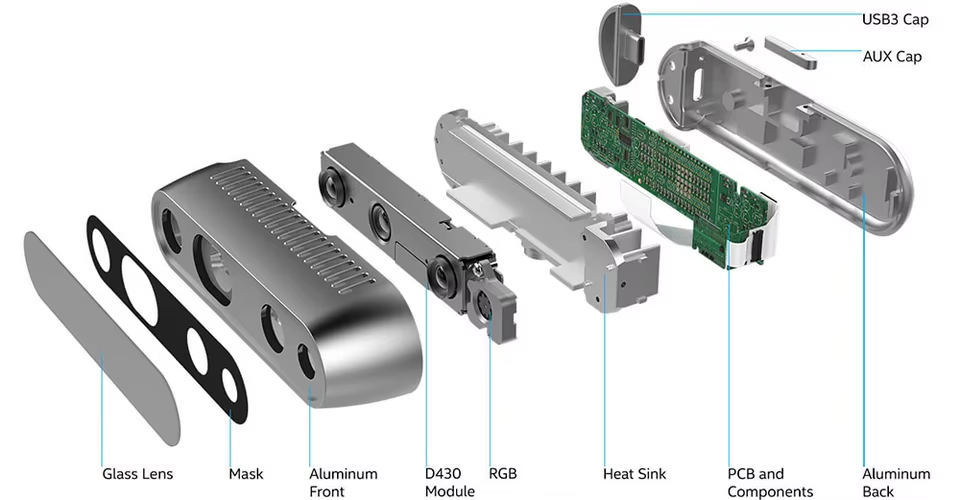
\includegraphics[scale=0.35]{images/rs_435i.png}}
\end{figure}


\begin{itemize}[nosep]
    \item Resolución de profundidad de hasta $1280 \times 720$ píxeles.
    \item Rango ideal de operación entre $0.3~\mathrm{m}$ y $3~\mathrm{m}$.
    \item Cámara RGB de $2~\mathrm{MP}$ con resolución de hasta $1920 \times 1080$ píxeles a $30~\mathrm{fps}$.
    \item Campo de visión del canal RGB de $69^\circ \times 42^\circ$.
    \item IMU Bosch BMI055 de 6 ejes, compuesta por acelerómetro a 200 Hz y un giroscopio a 100 Hz.
    \item Sincronización temporal de las muestras inerciales con los datos de profundidad mediante marcas de tiempo proporcionadas por el hardware.
    \item Conexión mediante USB-C 3.1 Gen 1.
    \item Dimensiones aproximadas de $90~\mathrm{mm} \times 25~\mathrm{mm} \times 25~\mathrm{mm}$.
\end{itemize}

La estación de tierra consta de un ordenador HP Probook, con un procesador intel core ULTRA 7, 32 GB de RAM y una gráfica 
NVIDIA GeForce RTX 2050 donde se ejecuta el programa de navegación autónoma.


\section{Resumen de algoritmia utilizada}

En esta sección se presenta una visión general de los principales módulos algorítmicos empleados en el sistema de navegación 
autónoma. El objetivo es describir de forma resumida el flujo completo de procesamiento, desde la recepción de los datos 
sensoriales hasta el envío de comandos de velocidad al UAV. Cada uno de estos bloques se desarrollará con mayor detalle en los 
apartados posteriores.

La recepción del canal visual se realiza mediante un flujo RTSP, lo que permite transmitir vídeo en tiempo real desde la 
plataforma aérea hasta la estación de tierra a través de Wi-Fi. Esta solución se ha seleccionado por su baja latencia, su 
compatibilidad con herramientas estándar de procesamiento de vídeo y su capacidad para mantener un flujo continuo de imágenes 
sin necesidad de almacenar todos los datos en memoria.

A partir de la información visual e inercial recibida, se implementa un sistema de odometría visual-inercial, basado 
conceptualmente en el enfoque propuesto en RVIO2~\cite{huai2022square} y ~\cite{huai2024consistent}. Este módulo estima la pose relativa del UAV respecto al instante 
inicial mediante la combinación de imágenes y medidas de la IMU. Aunque la arquitectura y algunos fundamentos teóricos se inspiran 
en dicho trabajo, el código empleado en este proyecto ha sido desarrollado de forma propia y adaptado a las necesidades 
específicas del sistema.

De forma complementaria, el canal visual se procesa mediante Depth Anything 3~\cite{overview-da}, utilizado como estimador de profundidad 
monocular. La información de profundidad obtenida permite generar una representación aproximada del entorno, que posteriormente 
se emplea en el módulo de evitación de obstáculos.

El sistema de planificación se divide en dos niveles. En primer lugar, el planificador global implementa una estrategia básica de 
tipo \textit{go-to}, encargada de generar una trayectoria de referencia hacia los \textit{waypoints} definidos por el usuario. En 
segundo lugar, el planificador local utiliza una variante tridimensional del algoritmo \textit{Pure Pursuit}, basado en~\cite{pp3d}, que permite adaptar 
la dirección de avance del UAV en función de la trayectoria global y de la información local del entorno.

Finalmente, las referencias generadas por el planificador local se introducen en un controlador PID, encargado de calcular los 
comandos de velocidad lineal y angular necesarios para guiar el UAV. Estos comandos se envían posteriormente al controlador de 
vuelo mediante comunicación UDP, cerrando así el ciclo de navegación.